\documentclass[10pt, landscape]{article}
\usepackage[scaled=0.92]{helvet}
\usepackage{calc}
\usepackage{multicol}
\usepackage{ifthen}
\usepackage[a4paper,margin=3mm,landscape]{geometry}
\usepackage{amsmath,amsthm,amsfonts,amssymb}
\usepackage{color,graphicx,overpic}
\usepackage{hyperref}
\usepackage{newtxtext} 
\usepackage{enumitem}
\usepackage{amssymb}
\usepackage[table]{xcolor}
\usepackage{vwcol}
\usepackage{tikz}
\usetikzlibrary{arrows.meta}
\usetikzlibrary{calc}
\usepackage{mathtools}
\usepackage{nicematrix}
%For pictures / figures
\usepackage{color,graphicx,overpic}
\graphicspath{ {./images/} }
% for relations
\usepackage{cancel}
\usepackage{ mathrsfs }
\graphicspath{ {./images/} }
\setlist{nosep}


\pdfinfo{
  /Title (CG2111A-Midterm.pdf)
  /Creator (TeX)
  /Producer (pdfTeX 1.40.0)
  /Author (Seamus)
  /Subject (Example)
  /Keywords (pdflatex, latex,pdftex,tex)}

% Turn off header and footer
\pagestyle{empty}

\newenvironment{tightcenter}{%
  \setlength\topsep{0pt}
  \setlength\parskip{0pt}
  \begin{center}
}{%
  \end{center}
}

% redefine section commands to use less space
\makeatletter
\renewcommand{\section}{\@startsection{section}{1}{0mm}%
                                {-1ex plus -.5ex minus -.2ex}%
                                {0.5ex plus .2ex}%x
                                {\normalfont\large\bfseries}}
\renewcommand{\subsection}{\@startsection{subsection}{2}{0mm}%
                                {-1explus -.5ex minus -.2ex}%
                                {0.5ex plus .2ex}%
                                {\normalfont\normalsize\bfseries}}
\renewcommand{\subsubsection}{\@startsection{subsubsection}{3}{0mm}%
                                {-1ex plus -.5ex minus -.2ex}%
                                {1ex plus .2ex}%
                                {\normalfont\small\bfseries}}%
\renewcommand{\familydefault}{\sfdefault}
\renewcommand\rmdefault{\sfdefault}
% makes nested numbering (e.g. 1.1.1, 1.1.2, etc)
\renewcommand{\labelenumii}{\theenumii}
\renewcommand{\theenumii}{\theenumi.\arabic{enumii}.}
\renewcommand\labelitemii{•}
%  for logical not operator
\renewcommand{\lnot}{\mathord{\sim}}
\renewcommand{\bf}[1]{\textbf{#1}}
\newcommand{\abs}[1]{\vert #1 \vert}
\newcommand{\Mod}[1]{\ \mathrm{mod}\ #1}

\makeatother
\definecolor{myblue}{cmyk}{1,.72,0,.38}
\everymath\expandafter{\the\everymath \color{myblue}}
% Define BibTeX command
\def\BibTeX{{\rm B\kern-.05em{\sc i\kern-.025em b}\kern-.08em
    T\kern-.1667em\lower.7ex\hbox{E}\kern-.125emX}}
\let\iff\leftrightarrow
\let\Iff\Leftrightarrow
\let\then\rightarrow
\let\Then\Rightarrow

% Don't print section numbers
\setcounter{secnumdepth}{0}

\setlength{\parindent}{0pt}
\setlength{\parskip}{0pt plus 0.5ex}
%% this changes all items (enumerate and itemize)
\setlength{\leftmargini}{0.5cm}
\setlength{\leftmarginii}{0.5cm}
\setlist[itemize,1]{leftmargin=2mm,labelindent=1mm,labelsep=1mm}
\setlist[itemize,2]{leftmargin=4mm,labelindent=1mm,labelsep=1mm}

%My Environments
\newtheorem{example}[section]{Example}
% -----------------------------------------------------------------------

\begin{document}
\raggedright
\footnotesize
\begin{multicols}{4}


% multicol parameters
% These lengths are set only within the two main columns
\setlength{\columnseprule}{0.25pt}
\setlength{\premulticols}{1pt}
\setlength{\postmulticols}{1pt}
\setlength{\multicolsep}{1pt}
\setlength{\columnsep}{2pt}

\begin{center}
    \fbox{%
        \parbox{0.8\linewidth}{\centering \textcolor{black}{
            {\Large\textbf{CG2111A Midterm}}
            \\ \normalsize{AY24/25 sem 2}}
            \\ {\footnotesize \textcolor{myblue}{github.com/mendax1234}} 
        }%
    }
\end{center}
\section{GPIO Programming}
\begin{enumerate}
    \item \textbf{Pin Mapping Table}
    \begin{tabular}{|c|l|}
    \hline
    \textbf{Arduino Pin} & \textbf{Atmega 328 port and pin number} \\
    \hline
    0 & Port D, pin 0 \\
    \hline
    1 & Port D, pin 1 \\
    \hline
    2 & Port D, pin 2 \\
    \hline
    3 & Port D, pin 3 (OC2B)\\
    \hline
    4 & Port D, pin 4 \\
    \hline
    5 & Port D, pin 5 (OC0B)\\
    \hline
    6 & Port D, pin 6 (OC0A)\\
    \hline
    7 & Port D, pin 7 \\
    \hline
    8 & Port B, pin 0 \\
    \hline
    9 & Port B, pin 1 (OC1A)\\
    \hline
    10 & Port B, pin 2 (OC1B)\\
    \hline
    11 & Port B, pin 3 (OC2A)\\
    \hline
    12 & Port B, pin 4 \\
    \hline
    13 & Port B, pin 5 \\
    \hline
    \end{tabular}
    \item \textbf{Source and Sink Current}
    \begin{itemize}
        \item \textbf{source current}: the current flows \textbf{out of} the pin
        \item \textbf{sink current}: the current flow \textbf{into} the pin
    \end{itemize}
    For the specific characteristics, see data sheet P365-P366.
    \item As long as the pin you want is set to 1, it will output HIGH, e.g. the LED will be turned on if it is connected.
    \item \textbf{Output or Input}: \textbf{Output or Input} regards to the Arduino itself. \textbf{Know whether it is output or input before doing anything!} 0 is used to configure input and 1 is used to configure output.
    \begin{itemize}
        \item \textbf{Read the Input value}: To read the value from an \textbf{input} pin, \texttt{PINB, PINC or PIND} contains the value you want.
    \end{itemize}
    \item \textbf{Bit Position}: The leftmost bit is Bit 7, the rightmost bit is Bit 0.
    \item Be aware of the \textbf{active-low / active-high} characteristic of the electrical component, and then think about what value you want to set to your output Arduino Pin.
    \item \textbf{Hex to Binary}
    \begin{center}
        \begin{tabular}{|c|c|}
            \hline
            Hex & Binary \\
            \hline
            A & 1010 \\
            \hline
            B & 1011 \\
            \hline
            C & 1100 \\
            \hline
            D & 1101 \\
            \hline
            E & 1110 \\
            \hline
            F & 1111 \\
            \hline
        \end{tabular}      
    \end{center}

\end{enumerate}

\section{Interrupts}
\begin{enumerate}
    \item \textbf{External Interrupts for Digital I/O}
    \begin{itemize}
        \item \textbf{INT0} and \textbf{INT1} are external interrupt pins (\textbf{PD2} and \textbf{PD3} on the ATmega328p).
        \item They are typically used for detecting changes\textbf{} in \textbf{external signals}, such as \textbf{button presses or sensor readings}.
        \item \textbf{INT0} and \textbf{INT1} can be triggered on specific \textbf{edge transitions} (rising or falling) or \textbf{low level signals}.
    \end{itemize}
    \item \textbf{Interrupt Mask: \texttt{cli()} and \texttt{sei()}}
    \begin{itemize}
        \item \textbf{\texttt{cli()}: Clear Interrupts}
        \item \textbf{\texttt{sei()}: Set Interrupts}
    \end{itemize}
    These two functions are used globally in for example \texttt{setup()} in the ATmega328p.
    \item \textbf{\texttt{volatile} keyword}
    \begin{itemize}
        \item TLDR, Always declare GLOBAL variables that are changed by ISRs to be \texttt{volatile}
    \end{itemize}
    \item \textbf{Calculating Transfer Time}
    \begin{itemize}
        \item \textbf{Polling}: The key for polling calculation is to calculate the \textbf{total clock cycles} the CPU spends in the \textbf{polling loop} while waiting for each byte to be ready. (a.k.a, \textbf{In Polling, we are more interested in the cycles wasted between reading each byte}) We ignore the cycles taken to read each byte.
        \item \textbf{Interrupts}: The key for interrupt calculation is to calculate the \textbf{total clock cycles} required to \textbf{handle each interrupt}, which typically \textbf{processes one byte}.
        \item \textbf{DMA}: The key for DMA calculation is to calculate the CPU cycles spent on setting up the DMA transfer, which can then transfer multiple bytes without further CPU intervention.
    \end{itemize}
    \item \textbf{Every pin has an Interrupt, but not each pin has an unique interrupt}. The 23 \texttt{PCINT} are grouped into 3 groups and all lines in the same group will trigger the execution of the \textbf{same} ISR.
    \item \textbf{Nested Interrupt}:
    \begin{itemize}
        \item It is \textbf{not enabled by default}
        \item If \textbf{enabled and triggered}, the interrupt may hand control back to ISR (not necessarily to \texttt{main}). 
    \end{itemize}
    \item \textbf{Interrupt Priority}: The \textbf{lower the address the higher the priority level}.
    \item \textbf{Context Switch}: Always remember to consider the \textbf{context switch}!
    
\end{enumerate}

\section{PWM}
\begin{enumerate}
    \item When the question has \textbf{PWM}, the Timer/Counter Module is by default using \textbf{Phase-Correct Mode}.
    \item The \textbf{default unit} for \textbf{period} is \textbf{seconds}. This means when you convert period to frequency, you must convert period to seconds first.
    \item In Phase Correct Mode, the \texttt{OCRnA} value is \textbf{always updated} when the TC counts to \textbf{TOP}.
    \item The two output compare pins can be set to generate PWM waveform together. e.g., set \texttt{OCR0A} will set the duty cycle for \texttt{OC0A}, set the \texttt{OCR0B} will set the duty cycle for \texttt{OC0B}.
    \item \textbf{Always check the \texttt{TCCRnA/B}'s \texttt{COM0A/B[1:0]} mode and draw the corresponding waveform to derive the duty cycle! Since it may affect the duty cycle!!!}
\end{enumerate}

\section{Timer}
\begin{enumerate}
    \item When the question has \textbf{Timer}, the Timer/Counter Module is by default using \textbf{CTC Mode}.
    \item \textbf{Timer Resolution vs. Timer Frequency}
    \begin{itemize}
        \item The \textbf{timer frequency} ($\frac{\text{F}_\text{clk}}{\text{P}}$) tells you \textbf{how many times the counter increments per second}. Its unit is \textbf{Hertz} (Hz).
        \item The \textbf{timer resolution} ($\frac{1}{\text{Timer Frequency}}$) tells you \textbf{how much time each increment takes}. Its unit is \textbf{seconds} (s).
    \end{itemize}
    \item \textbf{Interval}: Interval refers to the \textbf{time period between consecutive events} or \textbf{triggers}.
    \item \textbf{Waveform Period/Frequency calculation}
    \begin{itemize}
        \item When you know \texttt{OCRnA} value and want to use it to calculate \textbf{period/frequency of the waveform} you want to generate, \textbf{+1 and then times the timer resolution}.
        \item When you know the\textbf{ period/frequency of the waveform} you want to generate and want to use it to calculate the \texttt{OCRnA} value, \textbf{-1 and then times the timer resolution}.
    \end{itemize}
    \item \textbf{The intermediate value $V$}: $V-1=\texttt{OCRnA}$. When rounding the $V$ value, we always \textbf{round up}.
\end{enumerate}

\section{ADC}
\begin{enumerate}
    \item \textbf{Nyquist Theorem}: Signals should be sampled with \textbf{at least twice as fast as the highest frequency content of the signal}.
    \item \textbf{ADC Sampling Rate}: The \textbf{ADC sampling rate} refers to the \textbf{number of samples per second}. It is also called the \textbf{sample rate}. The unit of sampling rate is \textbf{samples per second} or \textbf{Hertz}. However, we know that \textbf{Hertz is the unit of frequency}. Therefore, the \textbf{sampling rate} can be also referred to as \textbf{sampling frequency}.
    \item In the \textbf{PRR}, the \textbf{PRADC} should be written to 0 to enable the ADC conversion!
\end{enumerate}

\section{USART}
\begin{enumerate}
    \item \textbf{Parity Bit}: The UART parity bit is set up when the \textbf{transmitting device is preparing to send data}. It is \textbf{not set in the receiver}. The receiver just receives the data the transmitter sends and \textbf{uses} the parity bit to check whether an error occurs.
    \begin{itemize}
        \item \textbf{2D Parity Bit}:
        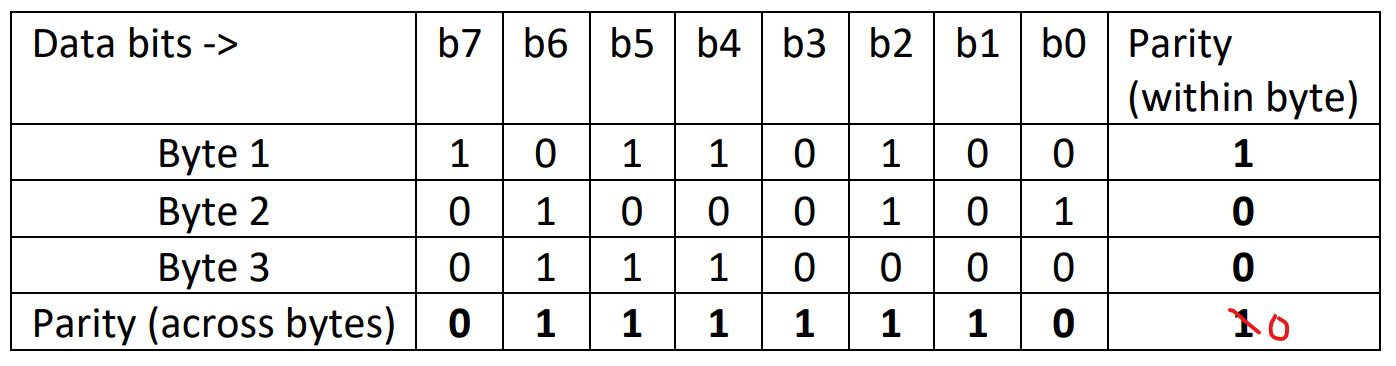
\includegraphics[width=1\linewidth]{images/2D-Parity-Bit.png}
        \begin{itemize}
            \item The last bit of the \textbf{parity (across bytes)} is calculated \textbf{across the last column, not using the last row!}
            \item When looking at such table, find \textbf{which column and which row} may be wrong, if there are multiple rows and columns that are wrong, you can \textbf{only change one bit in a row or column once}!
        \end{itemize}
    \end{itemize}
    \item \textbf{Sending Data Frame using UART}: \textbf{what you send is what you get}. e.g. You send the start bit first, then the first bit received by the receiver will be the start bit.
    \item \textbf{UART Setup preparation}:
    \begin{itemize}
        \item Number of data bits - 5, 6, 7, 8 or 9. Standard is 8.
        \item Type of parity bits: None(N), Even(E), or Odd(O)
        \item Number of stop bits: 1 or 2.
        \item Bit rate: 1200, 2400, 4800, 9600, etc. 
    \end{itemize}
    \item \textbf{Baud Rate and Bit Rate}:
    \begin{itemize}
        \item \textbf{Baud rate}: \textbf{The number of symbols} that can be sent per second.
        \item \textbf{Bit rate}: \textbf{The number of bits} that can be sent per second.
        \item \textbf{Conversion}: $\text{Bit rate}=\text{Baud rate}\times\text{bits required to represent per symbol}$
    \end{itemize}
    \item \textbf{Circular Buffer}: It is the method we use to implement our buffer in USART. \\
    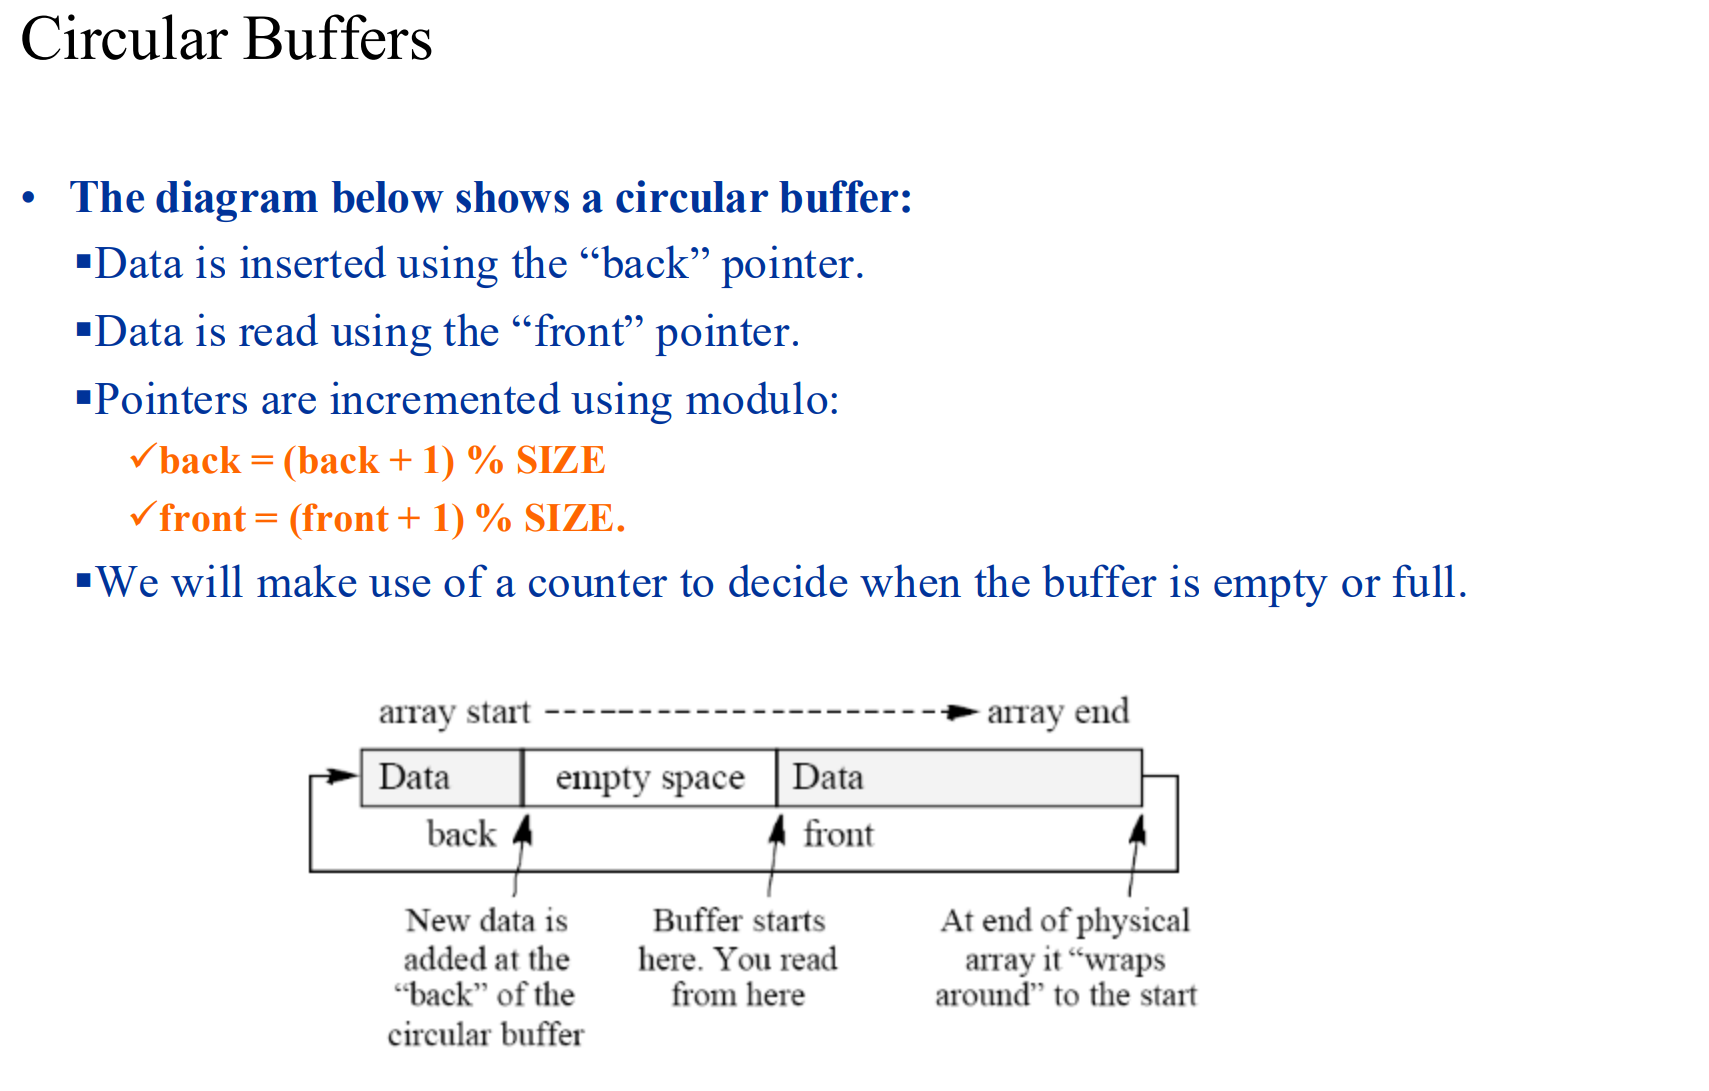
\includegraphics[width=1\linewidth]{images/circular-buffer.png}
\end{enumerate}

\section{Misc}
\begin{enumerate}
    \item \textbf{Unit Change (seconds)}:
    \begin{center}
        \begin{tabular}{|c|c|}
            \hline
            Unit & Seconds Equivalent \\
            \hline
            \textmu s (microsecond) & $10^{-6}$ s \\
            \hline
            ms (millisecond) & $10^{-3}$ s \\
            \hline
        \end{tabular}
    \end{center}
    \item Arduino \textbf{doesn't have an OS}.
    \item If you left shift a 1, for example by 10 position, and store the result into an 8-bit register. The final value will only \textbf{take the last 8 bits.}
    \item For a normal 8-bit register, if you increment the value in it by 1 all the time, it may wrap around or may not.
\end{enumerate}


\end{multicols}
\end{document}